% Options for packages loaded elsewhere
\PassOptionsToPackage{unicode}{hyperref}
\PassOptionsToPackage{hyphens}{url}
%
\documentclass[
  10pt,
  ignorenonframetext,
]{beamer}
\usepackage{pgfpages}
\setbeamertemplate{caption}[numbered]
\setbeamertemplate{caption label separator}{: }
\setbeamercolor{caption name}{fg=normal text.fg}
\beamertemplatenavigationsymbolsempty
% Prevent slide breaks in the middle of a paragraph
\widowpenalties 1 10000
\raggedbottom
\setbeamertemplate{part page}{
  \centering
  \begin{beamercolorbox}[sep=16pt,center]{part title}
    \usebeamerfont{part title}\insertpart\par
  \end{beamercolorbox}
}
\setbeamertemplate{section page}{
  \centering
  \begin{beamercolorbox}[sep=12pt,center]{part title}
    \usebeamerfont{section title}\insertsection\par
  \end{beamercolorbox}
}
\setbeamertemplate{subsection page}{
  \centering
  \begin{beamercolorbox}[sep=8pt,center]{part title}
    \usebeamerfont{subsection title}\insertsubsection\par
  \end{beamercolorbox}
}
\AtBeginPart{
  \frame{\partpage}
}
\AtBeginSection{
  \ifbibliography
  \else
    \frame{\sectionpage}
  \fi
}
\AtBeginSubsection{
  \frame{\subsectionpage}
}

\usepackage{amsmath,amssymb}
\usepackage{iftex}
\ifPDFTeX
  \usepackage[T1]{fontenc}
  \usepackage[utf8]{inputenc}
  \usepackage{textcomp} % provide euro and other symbols
\else % if luatex or xetex
  \usepackage{unicode-math}
  \defaultfontfeatures{Scale=MatchLowercase}
  \defaultfontfeatures[\rmfamily]{Ligatures=TeX,Scale=1}
\fi
\usepackage{lmodern}
\ifPDFTeX\else  
    % xetex/luatex font selection
\fi
% Use upquote if available, for straight quotes in verbatim environments
\IfFileExists{upquote.sty}{\usepackage{upquote}}{}
\IfFileExists{microtype.sty}{% use microtype if available
  \usepackage[]{microtype}
  \UseMicrotypeSet[protrusion]{basicmath} % disable protrusion for tt fonts
}{}
\makeatletter
\@ifundefined{KOMAClassName}{% if non-KOMA class
  \IfFileExists{parskip.sty}{%
    \usepackage{parskip}
  }{% else
    \setlength{\parindent}{0pt}
    \setlength{\parskip}{6pt plus 2pt minus 1pt}}
}{% if KOMA class
  \KOMAoptions{parskip=half}}
\makeatother
\usepackage{xcolor}
\newif\ifbibliography
\ifLuaTeX
  \usepackage{luacolor}
  \usepackage[soul]{lua-ul}
\else
  \usepackage{soul}
  \makeatletter
  \let\HL\hl
  \renewcommand\hl{% fix for beamer highlighting
    \let\set@color\beamerorig@set@color
    \let\reset@color\beamerorig@reset@color
    \HL}
  \makeatother
  
\fi
\setlength{\emergencystretch}{3em} % prevent overfull lines
\setcounter{secnumdepth}{-\maxdimen} % remove section numbering


\providecommand{\tightlist}{%
  \setlength{\itemsep}{0pt}\setlength{\parskip}{0pt}}\usepackage{longtable,booktabs,array}
\usepackage{calc} % for calculating minipage widths
\usepackage{caption}
% Make caption package work with longtable
\makeatletter
\def\fnum@table{\tablename~\thetable}
\makeatother
\usepackage{graphicx}
\makeatletter
\def\maxwidth{\ifdim\Gin@nat@width>\linewidth\linewidth\else\Gin@nat@width\fi}
\def\maxheight{\ifdim\Gin@nat@height>\textheight\textheight\else\Gin@nat@height\fi}
\makeatother
% Scale images if necessary, so that they will not overflow the page
% margins by default, and it is still possible to overwrite the defaults
% using explicit options in \includegraphics[width, height, ...]{}
\setkeys{Gin}{width=\maxwidth,height=\maxheight,keepaspectratio}
% Set default figure placement to htbp
\makeatletter
\def\fps@figure{htbp}
\makeatother
% definitions for citeproc citations
\NewDocumentCommand\citeproctext{}{}
\NewDocumentCommand\citeproc{mm}{%
  \begingroup\def\citeproctext{#2}\cite{#1}\endgroup}
\makeatletter
 % allow citations to break across lines
 \let\@cite@ofmt\@firstofone
 % avoid brackets around text for \cite:
 \def\@biblabel#1{}
 \def\@cite#1#2{{#1\if@tempswa , #2\fi}}
\makeatother
\newlength{\cslhangindent}
\setlength{\cslhangindent}{1.5em}
\newlength{\csllabelwidth}
\setlength{\csllabelwidth}{3em}
\newenvironment{CSLReferences}[2] % #1 hanging-indent, #2 entry-spacing
 {\begin{list}{}{%
  \setlength{\itemindent}{0pt}
  \setlength{\leftmargin}{0pt}
  \setlength{\parsep}{0pt}
  % turn on hanging indent if param 1 is 1
  \ifodd #1
   \setlength{\leftmargin}{\cslhangindent}
   \setlength{\itemindent}{-1\cslhangindent}
  \fi
  % set entry spacing
  \setlength{\itemsep}{#2\baselineskip}}}
 {\end{list}}
\usepackage{calc}
\newcommand{\CSLBlock}[1]{\hfill\break\parbox[t]{\linewidth}{\strut\ignorespaces#1\strut}}
\newcommand{\CSLLeftMargin}[1]{\parbox[t]{\csllabelwidth}{\strut#1\strut}}
\newcommand{\CSLRightInline}[1]{\parbox[t]{\linewidth - \csllabelwidth}{\strut#1\strut}}
\newcommand{\CSLIndent}[1]{\hspace{\cslhangindent}#1}

\newenvironment{figure*}{\begin{figure}}{\end{figure}}
\newenvironment{table*}{\begin{table}}{\end{table}}
\usepackage[english]{babel}
\usepackage{morewrites}
\newwrite\stuff
\usepackage{enumitem}
\setlist[description]{style=multiline,leftmargin=3cm,itemsep=20pt}
\usetheme{boxes}
\useoutertheme{metropolis}
\useinnertheme{circles}
\usecolortheme{dove}
\usefonttheme{serif}
\AtBeginDocument{\fontsize{8}{8}\selectfont}
\setbeamerfont{footnote}{size=\tiny}
\setbeamercolor{block title example}{bg=orange,fg=white}
\setbeamercolor{block body example}{bg=orange!20,fg=black}
\definecolor{fbblue}{RGB}{70,111,170}
\definecolor{fblightblue}{RGB}{230,234,240}
\setbeamercolor{frametitle}{bg=black,fg=white}
\setbeamercolor{framesubtitle}{bg=black,fg=white}
\setbeamercolor{section in head/foot}{bg=black,fg=white}
\setbeamercolor{subsection in head/foot}{bg=black,fg=white}
\makeatletter\newcommand{\@minipagerestore}{\setlength{\parskip}{1  em}}\makeatother
\makeatletter
\@ifpackageloaded{caption}{}{\usepackage{caption}}
\AtBeginDocument{%
\ifdefined\contentsname
  \renewcommand*\contentsname{Table of contents}
\else
  \newcommand\contentsname{Table of contents}
\fi
\ifdefined\listfigurename
  \renewcommand*\listfigurename{List of Figures}
\else
  \newcommand\listfigurename{List of Figures}
\fi
\ifdefined\listtablename
  \renewcommand*\listtablename{List of Tables}
\else
  \newcommand\listtablename{List of Tables}
\fi
\ifdefined\figurename
  \renewcommand*\figurename{Figure}
\else
  \newcommand\figurename{Figure}
\fi
\ifdefined\tablename
  \renewcommand*\tablename{Table}
\else
  \newcommand\tablename{Table}
\fi
}
\@ifpackageloaded{float}{}{\usepackage{float}}
\floatstyle{ruled}
\@ifundefined{c@chapter}{\newfloat{codelisting}{h}{lop}}{\newfloat{codelisting}{h}{lop}[chapter]}
\floatname{codelisting}{Listing}
\newcommand*\listoflistings{\listof{codelisting}{List of Listings}}
\makeatother
\makeatletter
\makeatother
\makeatletter
\@ifpackageloaded{caption}{}{\usepackage{caption}}
\@ifpackageloaded{subcaption}{}{\usepackage{subcaption}}
\makeatother
\makeatletter
\@ifpackageloaded{sidenotes}{}{\usepackage{sidenotes}}
\@ifpackageloaded{marginnote}{}{\usepackage{marginnote}}
\makeatother

\ifLuaTeX
  \usepackage{selnolig}  % disable illegal ligatures
\fi
\usepackage{bookmark}

\IfFileExists{xurl.sty}{\usepackage{xurl}}{} % add URL line breaks if available
\urlstyle{same} % disable monospaced font for URLs
\hypersetup{
  pdfauthor={Tom Cunningham},
  hidelinks,
  pdfcreator={LaTeX via pandoc}}


\author{}
\date{}

\begin{document}


\begin{frame}{}
\phantomsection\label{section}
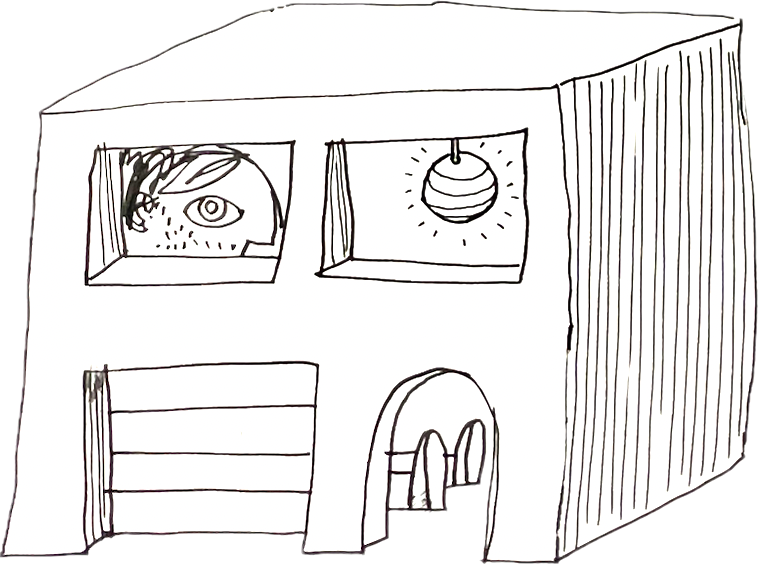
\includegraphics{images/2024-11-11-14-45-57.png}

\begin{description}
\tightlist
\item[Hi.]
It's lovely to be back around Facebook people :).
\end{description}
\end{frame}

\begin{frame}{Advertisements}
\phantomsection\label{advertisements}
\begin{description}
\item[Paper]
``\href{https://arxiv.org/abs/2402.06831}{What We Know About Using
Non-Engagement Signals in Content Ranking}''
\end{description}

\begin{description}
\item[Blog post]
``\href{https://tecunningham.github.io/posts/2023-01-31-social-media-suspensions-data.html}{Social
Media Suspensions of Prominent Accounts}''

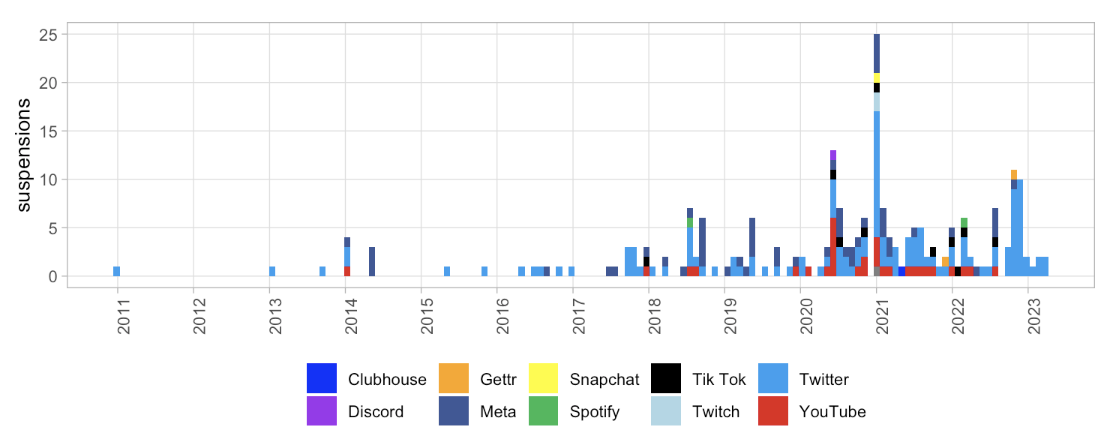
\includegraphics[width=5cm,height=\textheight]{images/2024-11-11-14-54-12.png}
\end{description}

\begin{description}
\tightlist
\item[Blog post]
``\href{https://tecunningham.github.io/posts/2023-07-27-meta-2020-elections-experiments.html}{How
Much has Social Media affected Polarization?}''

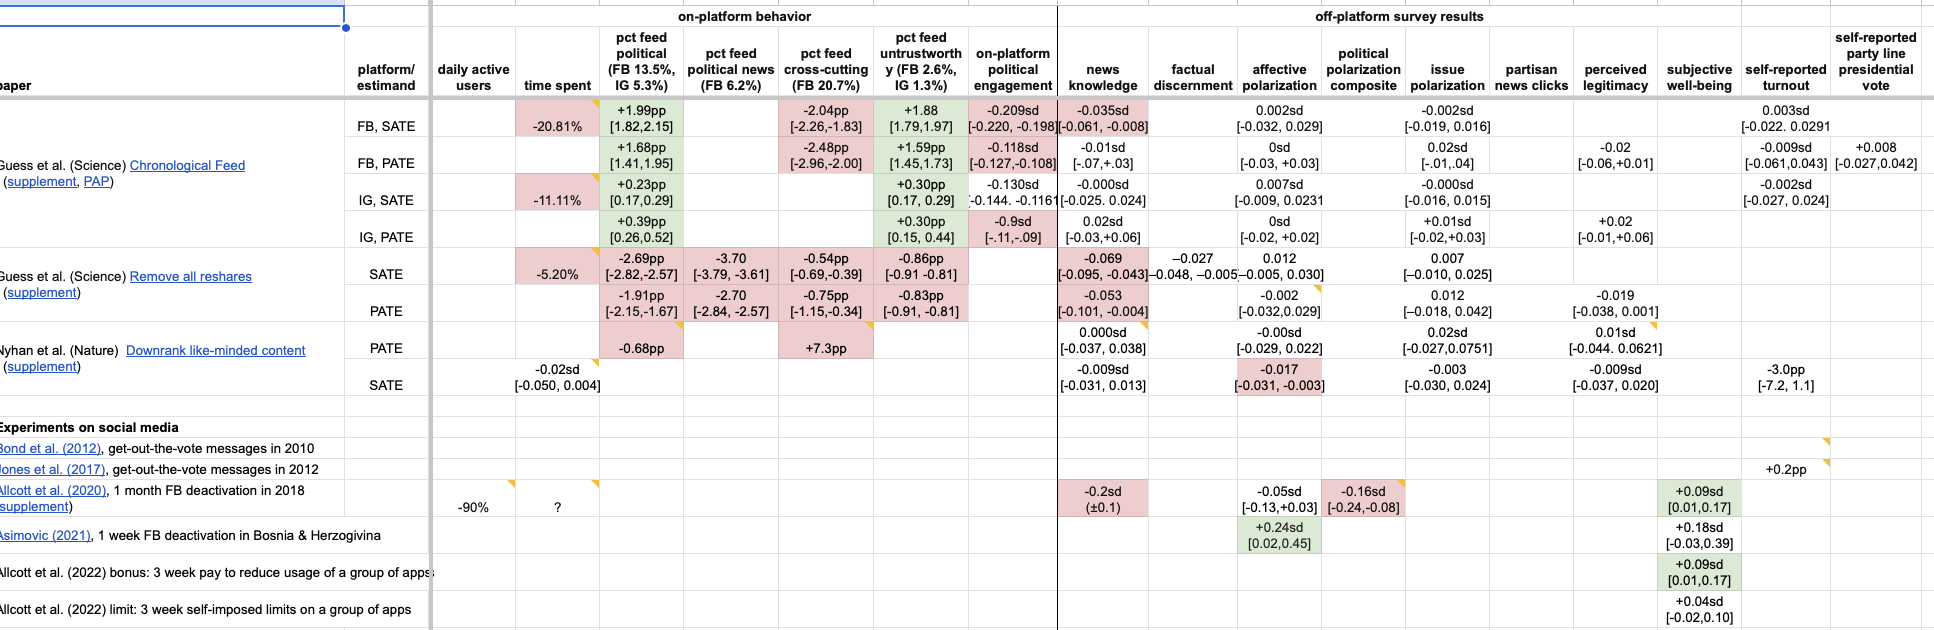
\includegraphics[width=5cm,height=\textheight]{images/2024-11-11-14-57-56.png}
\item[OpenAI work]
The economic impact of AI.
\end{description}
\end{frame}

\begin{frame}{Today}
\phantomsection\label{today}
\begin{description}
\item[What effect will AI have on content moderation and communication?]
I will talk about a dozen different aspects.
\end{description}

\vspace{2cm}

\begin{description}
\item[I will talk through some predictions.]
I add as much evidence and argument as I can, but often I will say ``it
seems reasonable to expect that\ldots{}''

Not sure how persuasive but I feel it's worth making concrete
predictions.
\end{description}
\end{frame}

\begin{frame}{Background on AI}
\phantomsection\label{background-on-ai}
\begin{description}
\tightlist
\item[AI is growing fast.]
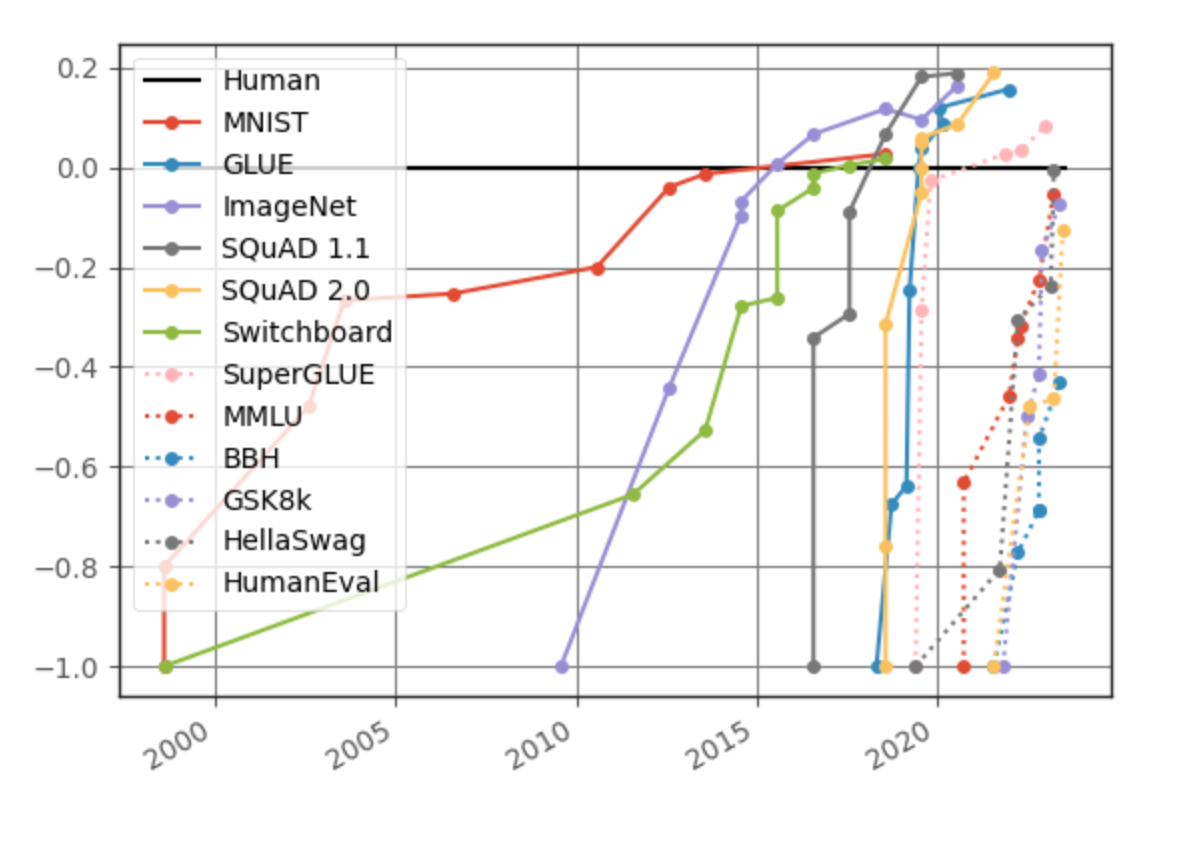
\includegraphics[width=3.125in,height=\textheight]{images/2023-09-19-09-55-57.png}
\item[AI can classify, but it can also synthesize.]
AI classification can approach human levels. But AI can also synthesize
new content, beyond the capabilities of any human.
\end{description}
\end{frame}

\begin{frame}{An Arms Race}
\phantomsection\label{an-arms-race}
\begin{description}
\item[We will be discussing adversarial equilibrium problems.]
Content moderation, spam filtering, misinformation. New models are
available to both sides, \& we want to know the equilibrium impact.
\item[An ``internal'' property of a message is a function solely of the
content.]
E.g. whether an image contains nudity, whether text contains hate
speech, whether a joke is funny. These properties hold independent of
any outside facts. AI classifiers are rapidly approaching human-level
accuracy for these properties and this means that platforms (and
governments) will be able to near-perfectly filter by internal
properties even if content-producers have access to the same technology.
\item[An ``external'' property of a message depends on some fact outside
the message's content.]
E.g. whether an image was computer-generated, whether a claim is true,
whether a message came from a specific person. Platforms will get better
at predicting external properties but they will be outpaced by motivated
actors who can manipulate fakes until they become indistinguishable from
genuine articles, and able to manipulate lies so they're
indistinguishable from the truth.
\end{description}
\end{frame}

\begin{frame}{Working on Formalizing these Arguments}
\phantomsection\label{working-on-formalizing-these-arguments}
\begin{description}
\tightlist
\item[Working on formalizing these arguments.]
Have been working with Ines Moreno de Barreda and Dan Quigley to try to
make these more formal. I feel it's an under-studied area.
\end{description}

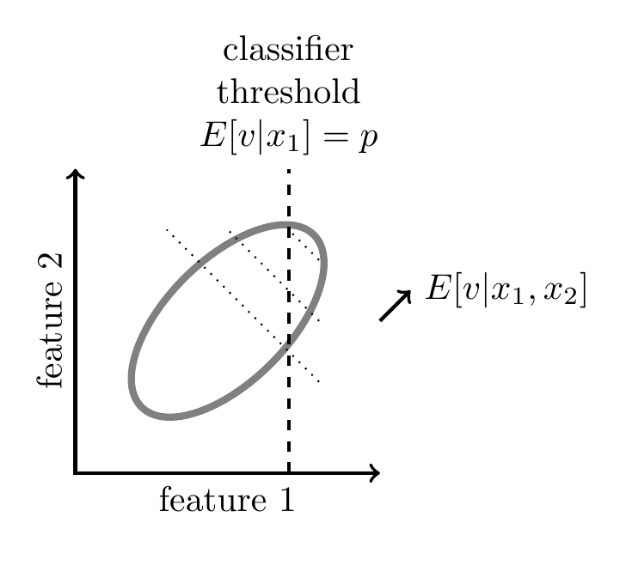
\includegraphics[width=3.125in,height=\textheight]{images/2024-11-12-09-39-14.png}
\end{frame}

\begin{frame}{The Prevalence of Policy-Violating Content Will Decline}
\phantomsection\label{the-prevalence-of-policy-violating-content-will-decline}
\begin{description}
\item[All large internet platforms use automated systems to detect
policy-violating content.]
All major platforms ban or suppress various types of content, e.g.~hate
speech, incitement to violence, nudity, graphic content. It has not been
practical to have a human review each message because the platforms have
a high volume of messages being sent with low latency. However automated
systems have always been used: early systems simply checked for the
appearance of prohibited words or matched against media databases, later
systems used classifiers trained on human labels. See a brief history of
automated content moderation
\href{https://tecunningham.github.io/posts/2023-11-18-history-automated-text-moderation.html}{here}.
\item[Simple classifiers have high offline accuracy.]
Simple classifiers which just look for the appearance of specific words
are often useful, e.g.~certain words and phrases are highly predictive
of whether text would be labelled as ``toxic'' or ``hate speech.''
However this method has many false positives (Chen (2022)) and false
negatives (Heiner (2022)).
\end{description}
\end{frame}

\begin{frame}{}
\phantomsection\label{section-1}
\begin{description}
\item[Simple classifiers are easily evaded.]
It is typically easy to alter a violating message such that humans still
think it is violating but the classifier does not. As a consequence the
accuracy of these classifiers looks much higher offline than online, as
users take steps to evade them.

\begin{itemize}
\tightlist
\item
  Gröndahl et al. (2018) note that hate speech detectors can easily be
  fooled if you ``insert typos, change word boundaries or add innocuous
  words.''
\item
  Han and Tsvetkov (2020) note that simple models are poor at detecting
  ``veiled toxicity'' which they define as including ``codewords, novel
  forms of offense, and subtle and often unintentional manifestations of
  social bias such as microaggressions and condescension.''
\item
  A. Lees et al. (2021) note that simple models are poor at detecting
  ``covert toxicity'' which includes ``types of toxicity that may not be
  immediately obvious. Covertly toxic comments may use obfuscation, code
  words, suggestive emojis, dark humor, or sarcasm \ldots{[}and{]}
  {[}m{]}icroaggressions.'' These papers evaluate models trained to
  identify \emph{context-independent} toxicity, i.e.~where the ground
  truth is human rating of the text alone without additional information
  on context or audience.
\end{itemize}
\item[LLM-based classifiers are approaching human levels of
performance.]
In August 2023 OpenAI described using GPT-4 as a content labeler (Weng,
Goel, and Vallone (2023)) and said ``{[}l{]}abeling quality by GPT-4 is
similar to human moderators with light training \ldots{} {[}h{]}owever,
both are still overperformed by experienced, well-trained human
moderators.''
\end{description}
\end{frame}

\begin{frame}{}
\phantomsection\label{section-2}
\begin{description}
\item[LLM-based classifiers handle adversarial cases well.]
Google's 2022 generation of text moderation models, which use
transformer-based LLMs, are able to correctly classify many types of
adversarial messages which are designed to evade simpler classifiers. A.
W. Lees et al. (2022) say their classifier performs well against
``code-switching, covert toxicity, emoji-based hate, human-readable
obfuscation, {[}and{]} distribution shift.'' Google's 2023 generation
spam classifier uses an embedding that is ``robust against typos and
character-level adversarial attacks'' (Bursztein et al.
(2023)).\footnote<.->{Arnaud Norman
  \href{https://bulkninja.notion.site/Email-Obfuscation-Rendered-almost-Ineffective-Against-ChatGPT-728fba1b948d42c6b8dfa73cb64984e4}{writes
  about} how algorithms to scrape email addresses are often easy to
  evade, by adding special characters or other obfuscations, but that
  ChatGPT can straight-forwardly decode most such obfuscations.}
\item[Better classifiers will lower prevalence even if they are
available to adversaries.]
Suppose an adversarial content-producer had access to the same
classifier that was used by the platform. The produced could keep
testing different variants of a violating post until they found a
variant that was truly violating, but not identified as violating by the
classifier, i.e.~a false negative. However as the platform's model
becomes more accurate there will be fewer possible false positives, and
so the task becomes relatively more time-consuming for the adversary,
and thus we should expect prevalence to decline.
\end{description}
\end{frame}

\begin{frame}{}
\phantomsection\label{section-3}
\begin{description}
\item[The prevalence of policy-violating content has declined
dramatically.]
Meta reports that the prevalence of nudity, bullying, hate speech, and
graphic content each declined by a factor of between 2 and 5 between
2017 and 2022, and that the share of identified-violating content that
was first identified by an ML model (``proactive rate'') is approaching
100\% for most categories. I think much of this decline can be
attributed to improvements in the quality of classifiers.\footnote<.->{It
  is important to remember that the ``proactive rate'' is the share of
  \emph{detected} content that is detected by AI, the share of
  \emph{violating} content that is detected by AI will certainly be
  significantly lower but is not generally reported. See Meta's
  \href{https://transparency.fb.com/data/community-standards-enforcement/}{Community
  Standards report} and
  \href{http://tecunningham.github.io/2023-01-31-social-media-suspensions-data.html\#meta-facebook-instagram}{my
  visualization of this data}.} Mark Zuckerberg has been making
predictions for a long time that human raters could be substituted with
AI. Although he was over-optimistic about the pace, I think he has been
largely correct, e.g.~in late 2018 he said ``through the end of 2019, we
expect to have trained our systems to proactively detect the vast
majority of problematic content.''\footnote<.->{Zuckerberg,
  \href{https://www.facebook.com/notes/751449002072082/}{``A Blueprint
  for Content Governance and Enforcement''}}
\end{description}

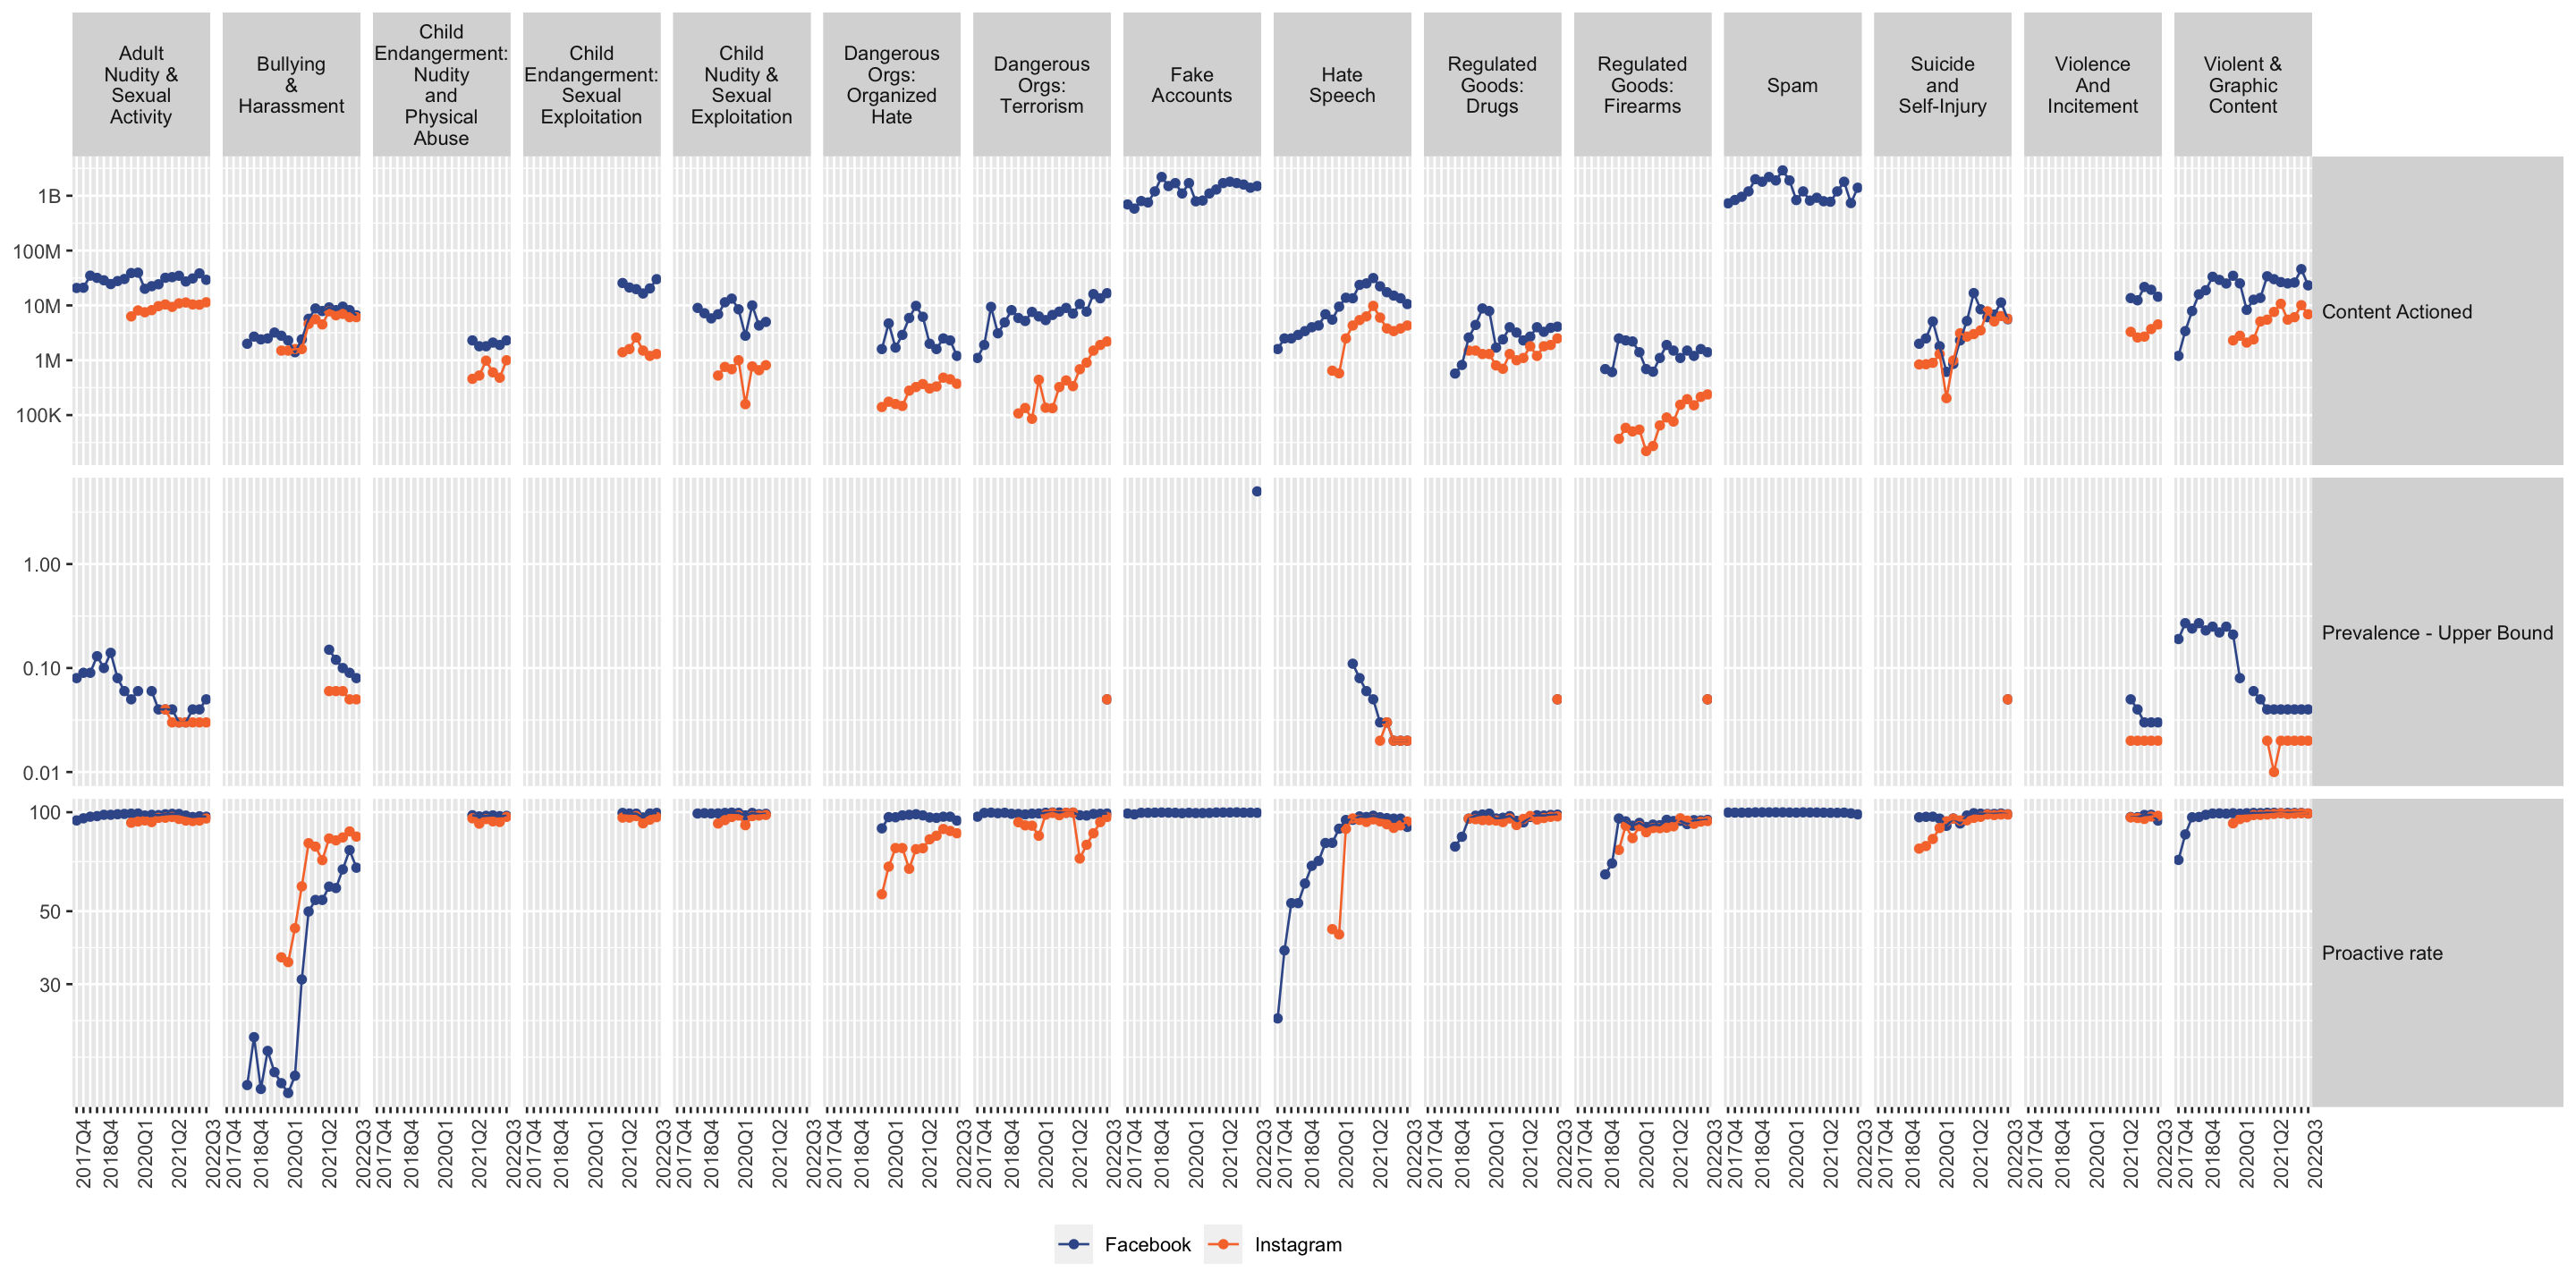
\includegraphics{./2023-01-31-social-media-suspensions-data_files/figure-html/unnamed-chunk-28-1.png}
\end{frame}

\begin{frame}{}
\phantomsection\label{section-4}
\begin{description}
\item[Employment of human moderators will likely decline.]
As computer accuracy improves fewer messages will need to be escalated
for human review, additionally fewer humans will be needed to label
training data.
\item[This prediction also applies to government monitoring and
censorship.]
Many governments use some kind of automated scanning tools to intercept
or censor messages based on their content, e.g.~the US's NSA and
Cybserspace Administration of China. Better AI will allow these agencies
to classify every post with reliability as high as if they had a human
read each one, thus we should expect obfuscation will become a much
less-effective workaround for censorship.
\end{description}
\end{frame}

\begin{frame}{}
\phantomsection\label{section-5}
\begin{description}
\item[This prediction would fail if there were hard limits on the
performance of AI.]
It's conceivable that there are ways of obfuscating content that will
remain difficult for an AI to identify for a long time. However even if
LLMs cannot identify violating content in real-time it seems likely they
could catch up quickly. Suppose humans invent new types of obfuscation,
e.g.~misspelling words in a particular way. An LLM which is continually
trained on human-labeled samples could likely learn the pattern and thus
force humans to continually adopt new patterns.
\item[Prevalence will never decline to exactly zero because it's
inherently noisy.]
An AI model can never perfectly predict human-rater evaluation because
humans are themselves noisy: there is both between-rater variation and
within-rater variation in labelling for any given piece of content. Thus
if the ground truth is human judgment then even an infallible classifier
could not be used to drive prevalence all the way to
zero.\footnote<.->{Strictly speaking: this will be true if no content
  has a probability of being labelled as positive by a human of exactly
  zero.}
\end{description}
\end{frame}

\begin{frame}{The Prevalence of \emph{Context-Specific} Violations Will
Increase}
\phantomsection\label{the-prevalence-of-context-specific-violations-will-increase}
\begin{description}
\item[Some messages have a violating significance only to their intended
audience.]
We can define a message as violating in one of two ways: (1) has a
violating significance to the average person (average citizen or average
user), or (2) has a violating significance to the intended audience of
that message.

I will define a ``contextual violation'' as a message that is violating
to its intended audience but not to the average person. This is stronger
than just having a double meaning where both meanings are clear to all
audiences. I am specifically talking about messages which are
interpreted in distinct ways by different audiences. Of course
contextual violations are often unstable, over time the average person
will often learn the contextual meaning.
\end{description}
\end{frame}

\begin{frame}{}
\phantomsection\label{section-6}
\begin{description}
\item[Many messages on social media use contextual
violations.\footnote<.->{A related phenomena is people using selective
  truths to give an impression that is false.}]
\begin{itemize}
\tightlist
\item[]
\item
  Saying ``globalist'' when your audience understands it to mean
  ``jewish''
\end{itemize}

\begin{itemize}
\tightlist
\item
  Saying the opposite of what is meant, e.g.~a bigot saying excessively
  positive things about an ethnic group, or a pro-anorexia poster making
  anti-anorexic statements sarcastically.
\end{itemize}

\begin{itemize}
\tightlist
\item
  Using euphemisms for illegal substances or illegal acts.
\end{itemize}

\begin{itemize}
\tightlist
\item
  Using emojis of eggplants and peaches with sexual connotations.
\end{itemize}

\begin{itemize}
\tightlist
\item
  Using photos without explicit nudity but which can be read as
  pornographic.
\end{itemize}
\item[Improved detection of violations is likely to cause substitution
towards contextual violations.]
As AI improves the ability to detect violations it seems likely that
there will be at least some substitution towards context-specific
violations, however as long as there is some cost to using a
contextual-violation then we would expect a less than one-for-one
substitution.
\end{description}
\end{frame}

\begin{frame}{}
\phantomsection\label{section-7}
\begin{description}
\item[Platforms could detect contextual violations if they wanted to.]
When doing human evaluation then platforms could either (1) provide
human raters with detail about the message's context and audience, or
(2) assign human raters to messages based on their experience with that
community.\footnote<.->{Platforms already have some policies that
  include context, e.g.~Facebook's
  \href{https://transparency.fb.com/policies/community-standards/bullying-harassment/}{``Bullying
  and Harassment policy''} bans ``repeatedly contacting someone in a
  manner that is unwanted or sexually harassing.''} Likewise AI models
could be trained to include rich representation of the context. An
additional advantage of adding context is that it can identify and
exempt posts that violate the letter but not the spirit of the policy.
\item[Platforms may not want to remove contextual violations.]
There are reasons why platforms may be reluctant to use context in
determining violations: it is more complex, and can lead to awkward PR
where the platform is shown to be censoring words and images have a
harmless interpretation.

Additionally platforms care both about being seen to restrict harmful
content, as well as about the actual harm prevented.
\end{description}
\end{frame}

\begin{frame}{}
\phantomsection\label{section-8}
\begin{description}
\item[Contextual violations have long existed in broadcast media.]
There have been many cases where contextual violations have been
tolerated: e.g.~newspapers would allow classified advertisments for
prostitutes if described as masseuses, vibrators if described as massage
wands, contraception if described as marital aids, and abortion if
described as
\href{https://slate.com/human-interest/2014/08/history-of-contraception-19th-century-classified-ads-for-abortifacients-and-contraceptives.html}{``removal
of obstructions''}. Thus it seems plausible that platforms will tolerate
a substantial amount of contextually-violating content to
remain.\footnote<.->{In Facebook's Marketplace it is prohibited to list
  guns for sale. As a consequence people began to list gun \emph{cases},
  with the understanding that a case was standing in for a gun. Facebook
  then updated their policy to prohibit selling gun cases. In turn
  people began to list gun stickers as stand-ins for guns. See WSJ
  reports from
  \href{https://www.wsj.com/articles/gun-sellers-are-sneaking-onto-facebooks-booming-secondhand-marketplace-11566315198}{2020}
  and
  \href{https://www.wsj.com/articles/gun-sellers-use-new-tactic-to-deal-on-facebook-marketplace-11598270872}{2021}.}
\item[Government censorship is unlikely to be constrained by
context-specific violations.]
Once a censor discovers that a term has an anti-government significance
in a certain context then they are likely to start censoring that term.
E.g. China has suppressed online mentions of
\href{https://www.bbc.com/news/blogs-china-blog-40627855}{Winnie the
Pooh} because it is associated with criticism of Xi Jinping, and in 2022
Hong Kong police arrested protestors for holding blank pieces of
paper.\footnote<.->{https://www.axios.com/2022/11/28/china-protests-blank-paper-covid}
\end{description}
\end{frame}

\begin{frame}{The Prevalence of Variants of Known-Violating Content Will
Decline}
\phantomsection\label{the-prevalence-of-variants-of-known-violating-content-will-decline}
\begin{description}
\item[Most platforms check content against databases of known-violating
content.]
The databases are often shared across platforms, known as ``signal
sharing'', e.g.~databases of illegal sexual media (PhotoDNA),
IP-protected content (Content ID), or terrorist recruitment content
(GIFCT).
\item[Existing equilibrium is cat-and-mouse obfuscation.]
Sophisticated uploaders obfuscate their content, e.g.~by adding noise,
and platforms expand their matching algorithms using fuzzy matching.
\item[Detecting variants of known content is subtly different from
detecting violating content.]
The difference between ``does this picture show a handsome face?'' and
``does this picture show Tom's face?''

The latter question becomes complicated: if a picture
\emph{coincidentally} looks like Tom, does it represent Tom? Much 20th
century philosophy has been written about these types of issues.
\end{description}
\end{frame}

\begin{frame}{}
\phantomsection\label{section-9}
\begin{description}
\item[It seems likely \emph{gratuitous} will violations to go to zero.]
Suppose someone wants to violate the policy just for the sake of
violating that policy, e.g.~they want to show a shocking image. Call
this ``gratuitous'' violations.

Currently the easiest way to do this is to first find a violating piece
of content, then obfuscate it.

If attackers can use AI synthesis they no longer need to find existing
violating content, they can synthesize new ones. The defensive technique
of checking against known-violating content becomes much worse.

However if defenders have AI recognition, then by the same argument as
above prevalence will go to zero.
\end{description}
\end{frame}

\begin{frame}{Platforms Will Not Be Able to Identify Bots from Their
Behavior}
\phantomsection\label{platforms-will-not-be-able-to-identify-bots-from-their-behavior}
\begin{description}
\item[Most online platforms struggle with automated users (bots) who are
disruptive in a variety of ways.]
One way of protecting against bots is with behavioral tests, e.g.~a
CAPTCHA test asking users an image-recognition task, or by using
on-platform behavior to detect whether a user is human. However
improvements in AI mean that computers have human-level performance on
image-recognition tasks, and can learn to imitate human-style behavior
patterns, thus it seems likely these behavioral tests will become
ineffective against sophisticated actors. Searles et al. (2023) finds
that most contemporary CAPTCHAs can be solved by computers with
higher-than-human accuracy.
\item[This does not imply that the prevalence of bots will increase.]
All platforms need some defense against bots so they will have to rely
relatively more on other forms of authentication, such as monetary
payment, offline identity credentials (government ID, credit card
number), hard-to-fake metadata (unique IP address, device ID), or
3rd-party identity provider (Sign in with Google, OpenID, Worldcoin).
Thus the barriers to signing up for a service, and especially posting on
it, will become higher, but the effect on equilibrium prevalence of bots
is ambiguous.

See \emph{Proof of Personhood} by OpenAI colleagues (Zoe Hitzig et al.).
\end{description}
\end{frame}

\begin{frame}{Platforms Will Find It Hard to Discriminate between Real
and Fake Media}
\phantomsection\label{platforms-will-find-it-hard-to-discriminate-between-real-and-fake-media}
\begin{description}
\item[In some cases the ground truth depends on properties outside the
content.]
I will refer to these properties as ``external'' in contrast to
``internal'' properties which depend only on the content such as whether
a picture depicts nudity. Some examples of external properties:

\begin{itemize}
\tightlist
\item
  Whether a piece of media was generated in the traditional way
  (photographing a scene, recording a sound), or has been manipulated or
  synthesized.
\item
  Whether text was written by a human.
\item
  Whether text was written by a specific person, e.g.~by Shakespeare.
\end{itemize}
\item[Advances in AI help both forgery-detection and forgery-creation.]
It is clear that a better statistical model of genuine artefacts will
help detect forgeries but it will also help create convincing forgeries.
\end{description}
\end{frame}

\begin{frame}{}
\phantomsection\label{section-10}
\begin{description}
\item[Determined forgers will be able to fool humans.]
It seems likely that the latter effect will dominate: it will gradually
become possible to camouflage computer-generated content such that
neither a computer nor a human could tell them apart. If the
content-producer has access to the platforms' model then they can keep
perturbing their fake media until it is labelled as non-fake.
\item[We cannot reliably discriminate between real and AI-generated
media.]
As of late 2023, programs to detect synthetically generated media have
relatively poor accuracy: OpenAI announced a model to detect LLM-created
text in January 2023 but then
\href{https://decrypt.co/149826/openai-quietly-shutters-its-ai-detection-tool}{shut
it down} in July because of poor performance. In June 2023 the NY Times
compared a variety of tools to detect computer-generated images and
found that with minimal effort they could all be
\href{https://www.nytimes.com/interactive/2023/06/28/technology/ai-detection-midjourney-stable-diffusion-dalle.html}{reliably
fooled}.
\end{description}
\end{frame}

\begin{frame}{}
\phantomsection\label{section-11}
\begin{description}
\item[The prevalence of synthetic media will increase on unmoderated
platforms.]
The major platforms have incentives to limit the prevalence of fake
media,\footnote<.->{The goals of platforms in content moderation are
  discussed in my note on ranking, Cunningham (2023).} and can control
the prevalence even without reliable classifiers. E.g. Meta and YouTube
dramatically decreased the prevalence of misinformation over 2016-2020
not primarily through real-time detection of whether a given claim is
false, but by (1) adjusting ranking to penalize publishers who tend to
circulate false claims; (2) punishing publishers who circulate
proven-false claims. Thus I do not expect overall prevalence of fake
factual media to substantially increase on the major platforms.
\end{description}
\end{frame}

\begin{frame}{Fake Media (Deepfakes) Will Not Have a Substantial
Influence on Politics}
\phantomsection\label{fake-media-deepfakes-will-not-have-a-substantial-influence-on-politics}
\begin{description}
\item[As synthetic media becomes common people will rely more on
provenance.]
As it becomes cheaper to manipulate and synthesize media then people are
likely to become more skeptical and rely relatively more on the
\emph{provenance} of information. Thus although synthetic media will
likely circulate I do not think it will have a substantial influence on
beliefs in equilibrium.
\item[It has always been easy to create misleading documents.]
It is not difficult to forge or alter documents, or edit video in a
misleading way. As a consequence mainstream media organizations
typically do not publish leaked materials unless they have either a
chain or provenance for the leaks or independent confirmation of their
content.
\end{description}
\end{frame}

\begin{frame}{}
\phantomsection\label{section-12}
\begin{description}
\item[Influential forgeries of documents have been historically rare.]
In an Appendix below I compile a simple dataset of politically
influential document leaks in the US over the past 25 years and estimate
around 10\% of them were based on forged materials.
\item[The quantity of false claims circulating on the internet is not
primarily constrained by the quality of their content.]
A great deal of false claims already circulate on the internet,
especially in loosely moderated parts: e.g.~by email, on Telegram,
4chan, Truth Social, WhatsApp, Twitter. It's not clear that the quality
of the faked media is an important constraint on the volume that
circulates.

It's not uncommon to find a clip of an interview with a politician
edited to make it appear that they are admitting to a crime or secret
agenda. If people already take what they see at face value then adding
deepfakes seems unlikely to change their opinions substantially.
Alternatively if people are skeptical and look for corroborating sources
then, again, deepfakes would be unpersuasive. It seems that deepfakes
would only be influential if there are a significant population who are
exposed to many lies but are not haded because the documentary evidence
is not sufficiently strong.
\end{description}
\end{frame}

\begin{frame}{Communication Will Migrate Towards Large Closed Platforms}
\phantomsection\label{communication-will-migrate-towards-large-closed-platforms}
\begin{description}
\item[Small platforms will be overrun with AI-created content.]
In particular, AI-created bots, spam, obfuscated violating content, and
fake media. This would imply that consumers will tend to migrate to
larger closed platforms with more effective defences, and which have
more restriction on participation. This continues a general movement
over the last 20 years of communication moving from small open platforms
(independent email, small forums, mailing lists, independent websites)
to large closed platforms (large email providers, large social media
platforms).
\item[People will rely more on established sources of truth.]
E.g. they will rely relatively more on Wikipedia, Community Notes, and
mainstream recognized media sources. The ordinary content-based signs of
trustworthiness will become less reliable: having a professional
website, well-edited text, well-argued reasoning, and documentary
evidence.
\end{description}
\end{frame}

\begin{frame}{}
\phantomsection\label{section-13}
\begin{description}
\item[People will rely more on cryptographic signing to verify
authenticity.]
I am not sure how strong this effect will be: it is generally more
efficient for an intermediary to verify authenticity of senders than for
users to do it themselves. I think we've seen that in other domains: (1)
PGP signing of email has been less important than email providers
filtering spam and phishing; (2) SSL certificates in browsers have been
less important than browsers giving warnings for suspected phishing
sites (e.g.~Google's \href{https://safebrowsing.google.com}{safe
browsing} database of sites with phishing or malware is used to give
warnings in Chrome and Safari).
\item[Pedigree will become more important in publication.]
As an editor accepting submissions (e.g.~an academic journal, a literary
magazine, a newspaper letters page) the quality of the work submitted is
typically correlated with more superficial features such as the
grammaticallity and the length. As it becomes easy to synthesize text
then those superficial features will become less informative about
quality and editors are likely to rely relatively more on hard-to-fake
signals like the pedigree of authors: what have they published before,
and which college the author went to.
\end{description}
\end{frame}

\begin{frame}{Entertainment will Become Largely Synthetic}
\phantomsection\label{entertainment-will-become-largely-synthetic}
\begin{description}
\item[A computer that can detect if a photo is pretty can also create a
pretty photo.]
A classifier that can detect whether a joke is funny should also be able
to generate funny jokes.{[}\^{}jokes{]} On average people spend around 3
hours per day watching entertainment (TV, YouTube, TikTok, Instagram).
It seems likely that trained models will be able to synthesize content
that is highly engaging though it's hard to anticipate what it will look
like.
\end{description}
\end{frame}

\begin{frame}{Things Will Get Weird}
\phantomsection\label{things-will-get-weird}
\begin{description}
\item[People will synthesize completely new violating images/videos.]
Thiel, Stroebel, and Portnoff (2023) say that, as of early 2023, less
than 1\% of child sexual abuse media (CSAM) appears to be synthetically
generated. However the ability to synthesize has been advancing rapidly,
``to the point that some images are only distinguishable from reality if
the viewer is very familiar with photography, lighting and the
characteristics of diffusion model outputs \ldots{} it is likely that in
under a year it will become significantly easier to generate adult
images that are indistinguishable from actual images.''
\item[Producers will synthesize content to sit on the \emph{edge} of a
category.]
If platforms take action whenever content passes some threshold then
adversarial actors will generate or perturb content such that it sits
right below the threshold. If a platform removes a photo whenever more
than 50\% of raters would say it depicts nudity then producers would
upload photos which 49\% of raters would say depicts nudity. People
would upload movies which \emph{almost} look like an existing
IP-protected movie, and students might submit essays that are close to
existing sources but don't quite trigger the plagiarism detector.
\end{description}
\end{frame}

\begin{frame}{Influential leaks of US political documents since 1997:}
\phantomsection\label{influential-leaks-of-us-political-documents-since-1997}
\begin{longtable}[]{@{}
  >{\raggedright\arraybackslash}p{(\columnwidth - 6\tabcolsep) * \real{0.4184}}
  >{\raggedright\arraybackslash}p{(\columnwidth - 6\tabcolsep) * \real{0.0408}}
  >{\raggedright\arraybackslash}p{(\columnwidth - 6\tabcolsep) * \real{0.1735}}
  >{\raggedright\arraybackslash}p{(\columnwidth - 6\tabcolsep) * \real{0.3673}}@{}}
\toprule\noalign{}
\endhead
Tripp Tapes & 1997 & audio & Tripp to Starr \\
\st{Iraq letters to Niger (``yellowcake'')} & 2002 & documents & Unknown
to Italians to CIA \\
\st{Bush military transcripts (``Killian'')} & 2004 & fax of 1970s memo
& Unknown to ret colonel to CBS \\
Abu Ghraib photos & 2004 & photos & Unknown to CBS \\
Baghdad Airstrike & 2007 & video & Chelsea Manning to Wikileaks \\
US Iraq war logs & 2010 & digital docs & Chelsea Manning to Wikileaks \\
US Diplomatic cables & 2010 & digital docs & Chelsea Manning to
Wikileaks \\
Romney Tape (``47\%'') & 2012 & audio & Bartender to Mother Jones \\
NSA Surveillance Leaks & 2013 & digital docs & Edward Snowden to the
Guardian, WaPo \\
DNC emails & 2016 & emails & Unknown to Wikileaks \\
Podesta emails & 2016 & emails & Unknown to Wikileaks \\
Colin Powell emails & 2016 & emails & Unknown to DCLeaks \\
Panama papers & 2016 & documents & Unknown to Süddeutsche Zeitung \\
Donald Trump Access Hollywood Tape & 2016 & video & Unknown to
Washington Post \\
China Cables & 2019 & digital docs & Unknown to the ICIJ \\
Hunter Biden laptop & 2020 & docs, audio, video & computer shop to
Giuliani to NY Post \\
Los Angeles Council call (``changuito'') & 2022 & audio & Unknown to
Reddit to LA Times \\
\bottomrule\noalign{}
\end{longtable}
\end{frame}

\begin{frame}{}
\phantomsection\label{section-14}
\phantomsection\label{refs}
\begin{CSLReferences}{1}{0}
\bibitem[\citeproctext]{ref-bursztein2023retvec}
Bursztein, Elie, Marina Zhang, Owen Vallis, Xinyu Jia, and Alexey
Kurakin. 2023. {``RETVec: Resilient and Efficient Text Vectorizer.''}
\url{https://arxiv.org/abs/2302.09207}.

\bibitem[\citeproctext]{ref-chen2022profanity}
Chen, Edwin. 2022.
\url{https://www.surgehq.ai/blog/are-popular-toxicity-models-simply-profanity-detectors}.

\bibitem[\citeproctext]{ref-cunningham2023ranking}
Cunningham, Tom. 2023. {``Ranking by Engagement.''}
\url{http://tecunningham.github.io/2023-04-28-ranking-by-engagement.html}.

\bibitem[\citeproctext]{ref-grondahl2018need}
Gröndahl, Tommi, Luca Pajola, Mika Juuti, Mauro Conti, and N. Asokan.
2018. {``All You Need Is "Love": Evading Hate-Speech Detection.''}
\url{https://arxiv.org/abs/1808.09115}.

\bibitem[\citeproctext]{ref-han2020fortifying}
Han, Xiaochuang, and Yulia Tsvetkov. 2020. {``Fortifying Toxic Speech
Detectors Against Veiled Toxicity.''} In \emph{Proceedings of the 2020
Conference on Empirical Methods in Natural Language Processing (EMNLP)},
7732--39. Online: Association for Computational Linguistics.
\url{https://doi.org/10.18653/v1/2020.emnlp-main.622}.

\bibitem[\citeproctext]{ref-heiner2022toxic}
Heiner, Scott. 2022. {``Real-World ML Failures: The Violence, Racism,
and Sexism Uncaught by Twitter's Content Moderation Systems.''}
\url{https://www.surgehq.ai/blog/25-examples-of-twitters-content-moderation-failures}.

\bibitem[\citeproctext]{ref-whitlocklees2022perspective}
Lees, Alyssa Whitlock, Vinh Q. Tran, Yi Tay, Jeffrey Scott Sorensen, Jai
Gupta, Donald Metzler, and Lucy Vasserman. 2022. {``A New Generation of
Perspective API: Efficient Multilingual Character-Level Transformers.''}
In. \url{https://dl.acm.org/doi/10.1145/3534678.3539147}.

\bibitem[\citeproctext]{ref-lees2021capturing}
Lees, Alyssa, Daniel Borkan, Ian Kivlichan, Jorge Nario, and Tesh Goyal.
2021. {``Capturing Covertly Toxic Speech via Crowdsourcing.''} In
\emph{Proceedings of the First Workshop on Bridging Human{--}Computer
Interaction and Natural Language Processing}, 14--20. Online:
Association for Computational Linguistics.
\url{https://aclanthology.org/2021.hcinlp-1.3}.

\bibitem[\citeproctext]{ref-searles2023empirical}
Searles, Andrew, Yoshimichi Nakatsuka, Ercan Ozturk, Andrew Paverd, Gene
Tsudik, and Ai Enkoji. 2023. {``An Empirical Study \& Evaluation of
Modern CAPTCHAs.''} \url{https://arxiv.org/abs/2307.12108}.

\bibitem[\citeproctext]{ref-thiel2023generative}
Thiel, David, Melissa Stroebel, and Rebecca Portnoff. 2023.
{``Generative ML and CSAM: Implications and Mitigations.''}

\bibitem[\citeproctext]{ref-weng2023gpt4moderation}
Weng, Lilian, Vik Goel, and Andrea Vallone. 2023. {``Using GPT-4 for
Content Moderation.''}
\url{https://openai.com/blog/using-gpt-4-for-content-moderation}.

\end{CSLReferences}
\end{frame}




\end{document}
